\documentclass{article}
\usepackage{graphicx}
\usepackage{float}

\title{IdentiFisher: \\ User Guide \\}



\author{
\Large McDonald, Christopher\\
\texttt{1312456} \\ \\
\Large Guo, Tian\\
\texttt{1327833} \\ \\
\Large Murray, Shandelle\\
\texttt{1303109} \\ \\
\Large Cheung, Ocean\\
\texttt{1316057} \\
}

\vfill
\date{\today}

\begin{document}
\maketitle

\newpage
\tableofcontents
\vfill
\noindent \\


\pagebreak
\section{Introduction}

\subsection{Purpose of Application}
The purpose of the IdentiFisher application is to identify a fish caught in a particular area
by searching a database of fish based on identifiable attributes. These attributes are easily distinguished by looking at the fish and include
colour, pattern, and shape. This application is designed for anyone who lacks the knowledge to distinguish a fish that they have caught and may be especially helpful for beginners.

\subsection{Developers}
The software system, IdentiFisher, is an Android application.
This system will be a utility application for anyone who fishes, either recreationally or
competivitely. It will service beginner to experienced fishers. IdentiFisher will allow
the user to provide information about a recently caught fish in order to attempt to identify what type
of fish it is. From there, it is able to collect data and track statistics concerning which types of fish have been caught in specific locations. The aim is to
build a global logging system that will provide percentage catch rate statistics by lake,
educate young, novice fishers, and integrate technology into a relatively non-technological field.


\section{Instructions}
This section will discuss the layout of each page of the application and each page's respective functions.
A walkthrough of how to complete possible tasks will also be presented.

\subsection{Main Page}
The main page controls the display of other pages and their respective functions. The user may navigate to the
appropriate page from the main page based on which function is needed. \\

\begin{figure}[H]
	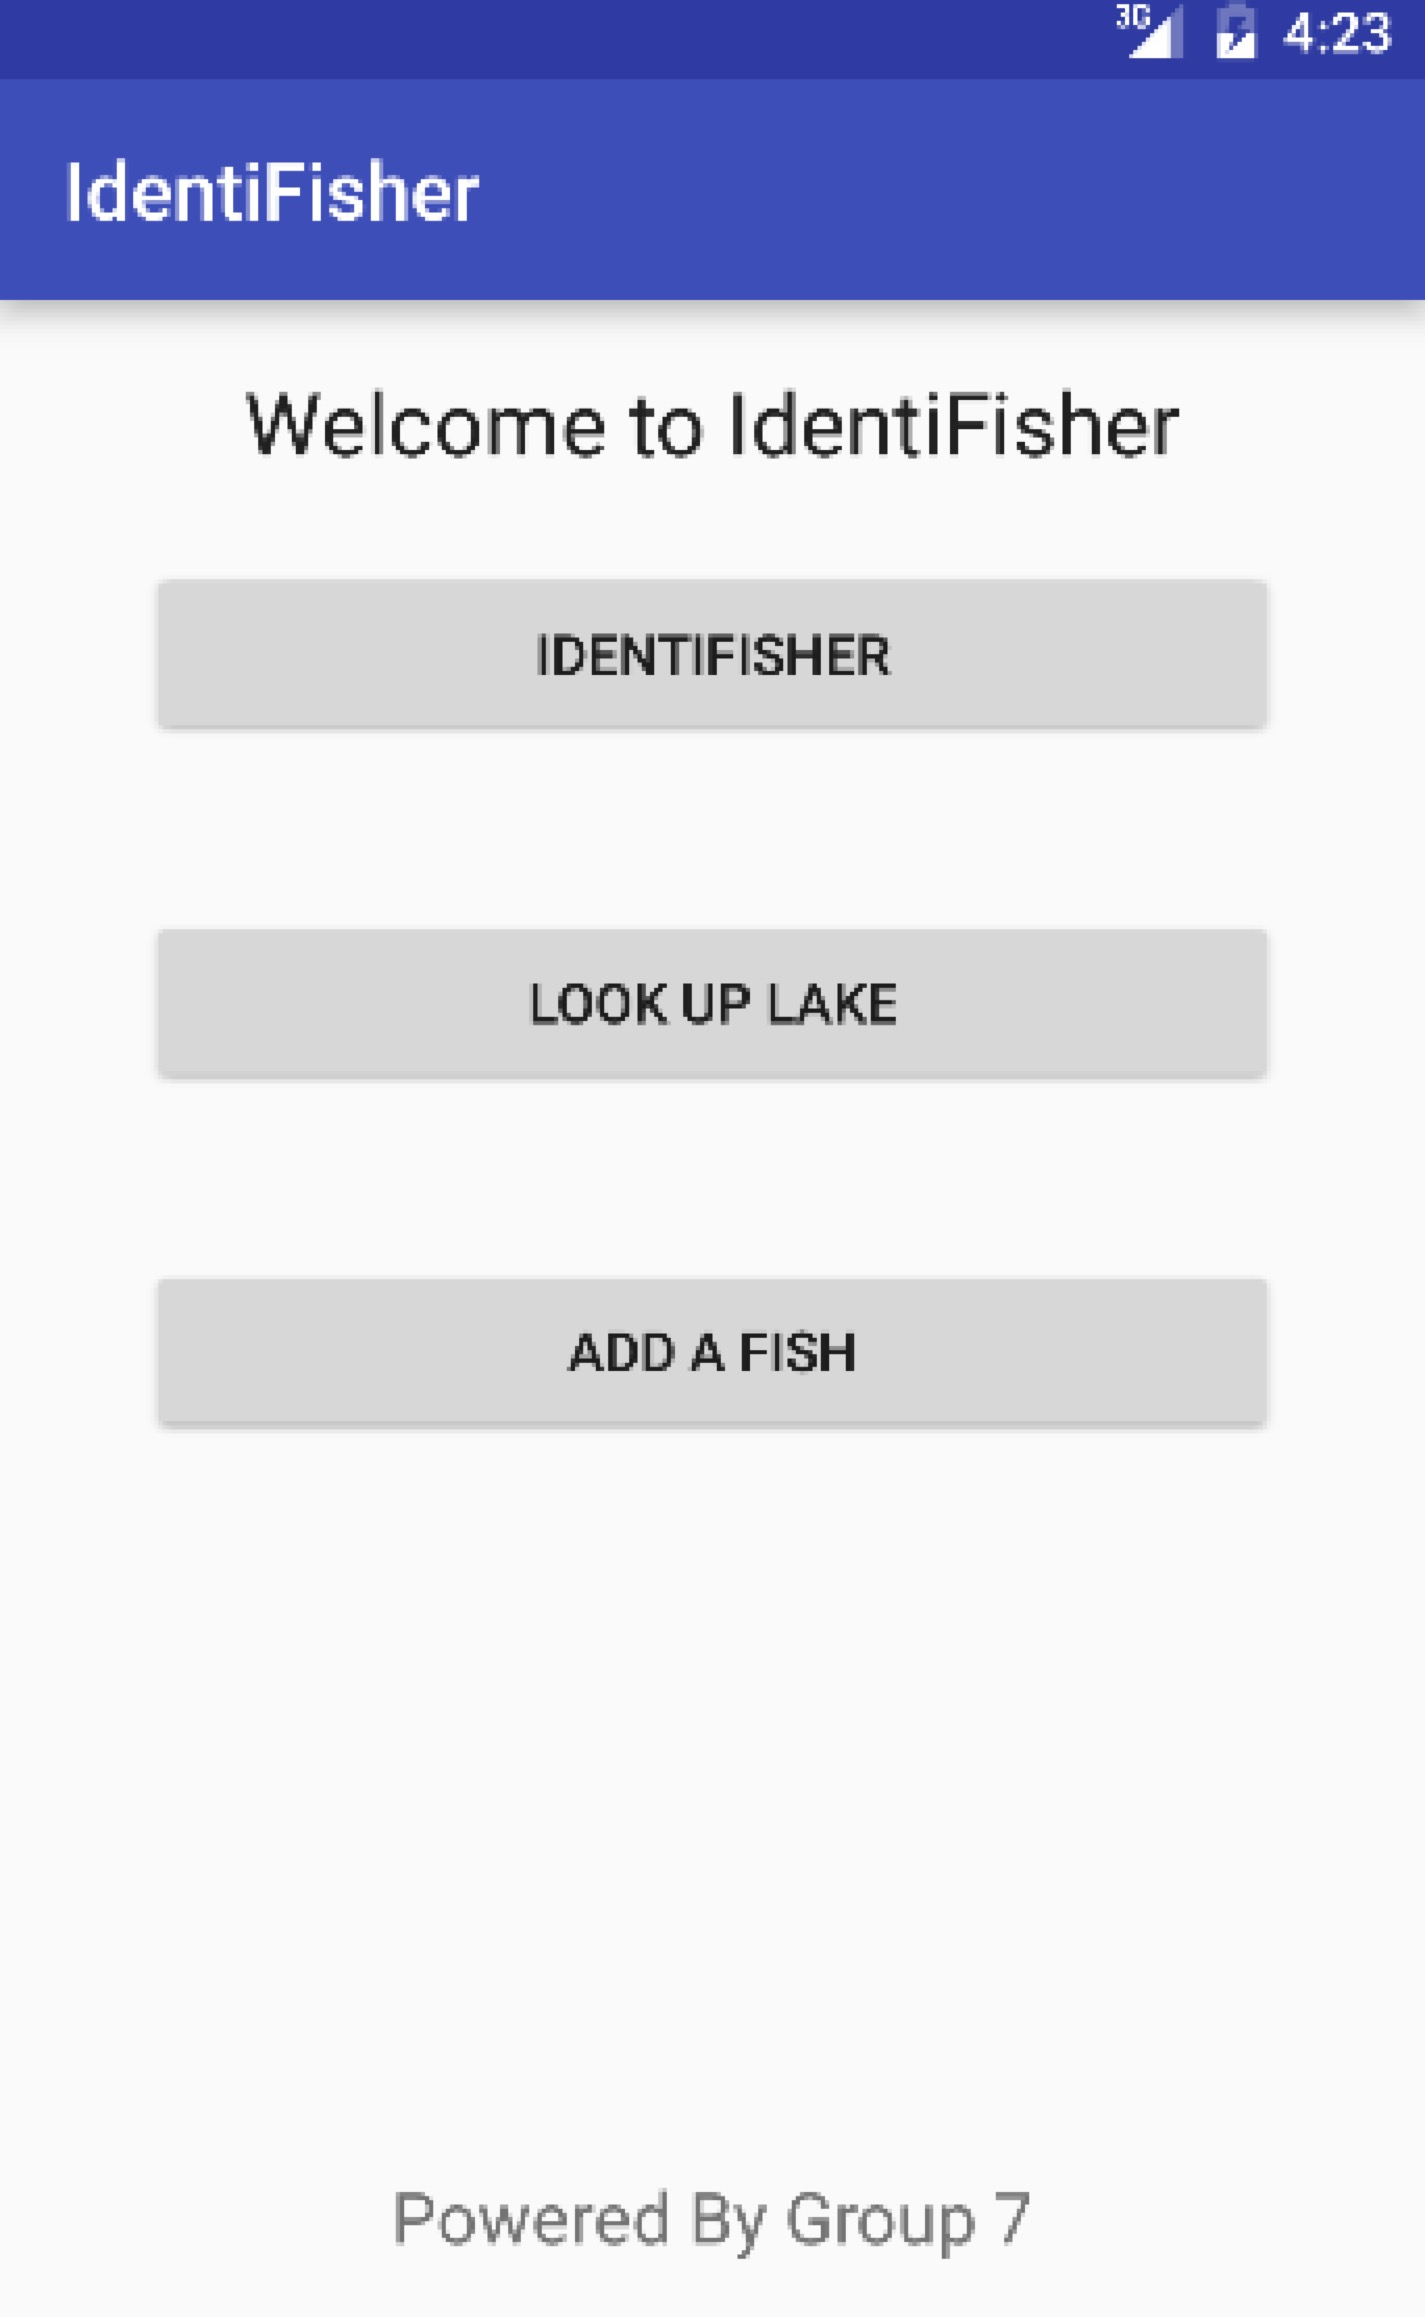
\includegraphics[scale=0.16]{Mainpage.png}
	\caption{Main page of IdentiFisher Application}
\end{figure}

The main page displays the name of the application as well as a welcome message at the top of the screen. There are three
buttons that, when pressed, will navigate to a different page. The  \textit{IDENTIFISHER} button will take the user to a page
where the user is able to select different properties of a fish that they wish to identify. The \textit{LOOK UP LAKE} button will navigate to a page where the
user may search for a lake near a certain location to find a list of possible fish in the area. The \textit{ADD A FISH} button will navigate
to a page where the user may add a fish and its location to the database of the application without going through the identification process.\\

\subsection{IDENTIFISHER Page}
The IDENTIFISHER page displays an instruction message at the top of the page: \textit{Please enter the following criteria}. There are three
drop-down menus representing colour, pattern, and shape of the fish respectively. There is an "IDENTIFY!" button towards the bottom of the page that the user can select in order to start the identification once the desired properties have been selected.\\

\begin{figure}[H]
	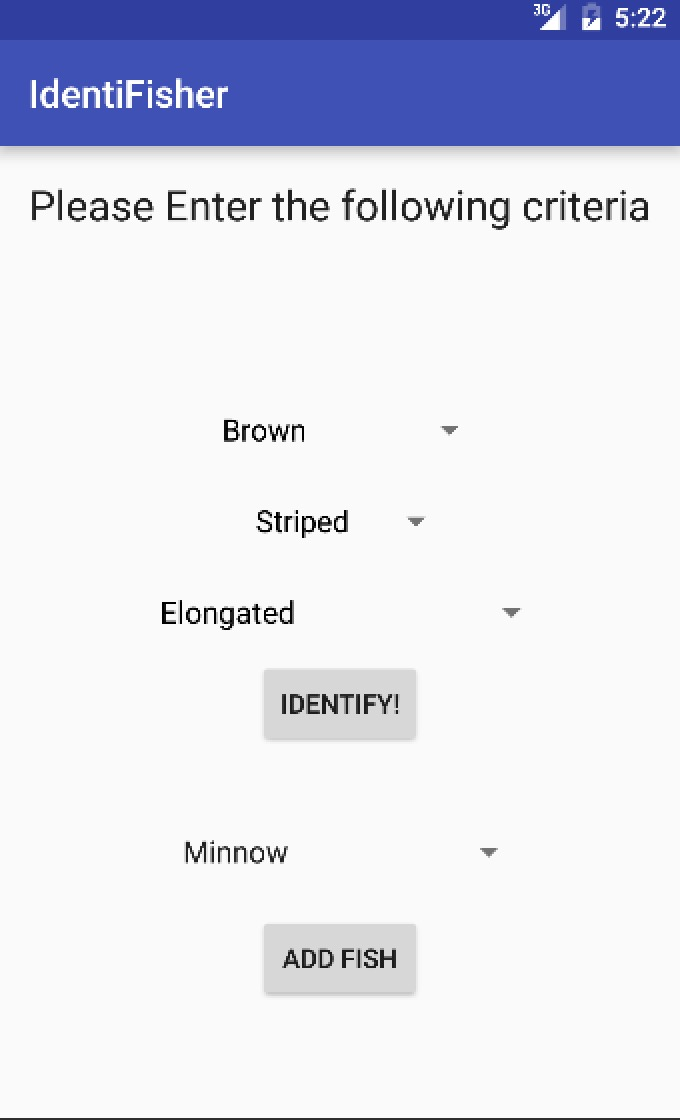
\includegraphics[scale=0.30]{IdentiFisher.png}
	\caption{IDENTIFISHER page of IdentiFisher Application}
\end{figure}

After selecting the "IDENTIFY!" button, the application will display the most probable types of fish. The user can also click on the drop-down
menu to display a list of other possible species of fish. Finally the user may add the fish to the database by pressing the \textit{ADD FISH} button.\\

\subsection{LOOK UP LAKE Page}
The LOOK UP LAKE page has a title as well as instructions prompting the user to input a location. There is a text field for input and a
\textit{FIND MY LAKE} button. Once the button is pressed having an input in the text field, the program will return a list of fish that can be found within the
region\\
\begin{figure}[H]
	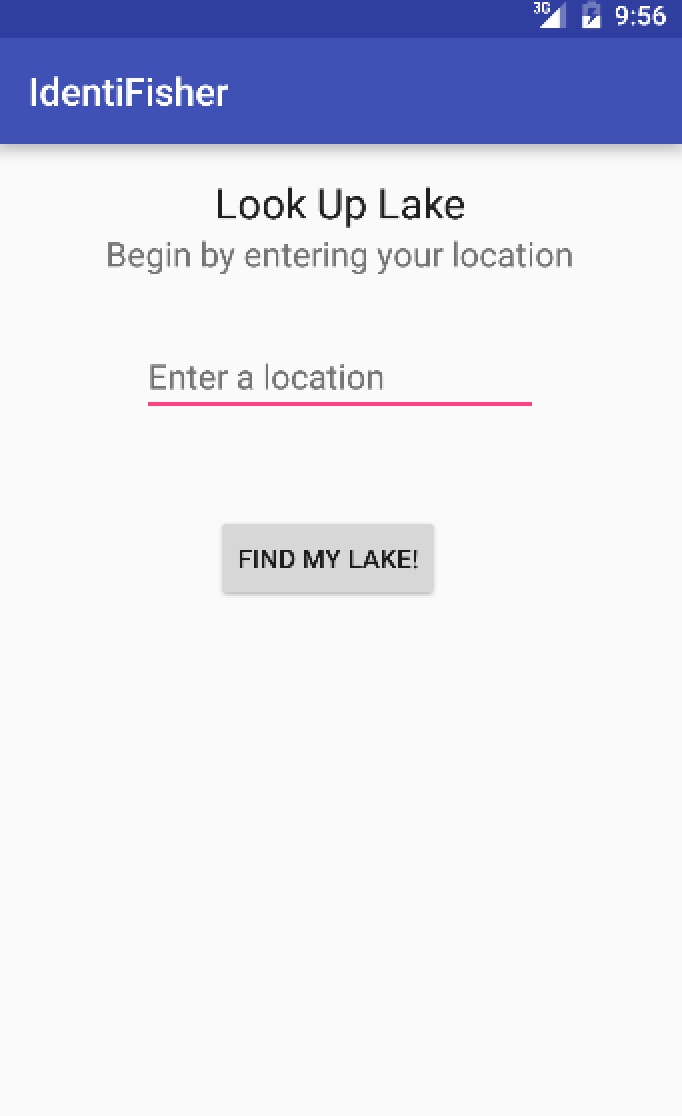
\includegraphics[scale=0.30]{Lookup.png}
	\caption{LOOK UP LAKE page of IdentiFisher Application}
\end{figure}

\subsection{ADD A FISH Page}
The top of the page displays the title as well as a message to help the user understand the function of the page. There is a text field to input the
location of the fish found. An example input is displayed in the text field: \textit{42 Wallaby Way, Sydney}. There is also a \textit{DETECT MY LOCATION} button
to use the current location of the device as input. There is a drop-down list of fish to choose from and an \textit{ADD FISH} button.\\
\begin{figure}[H]
	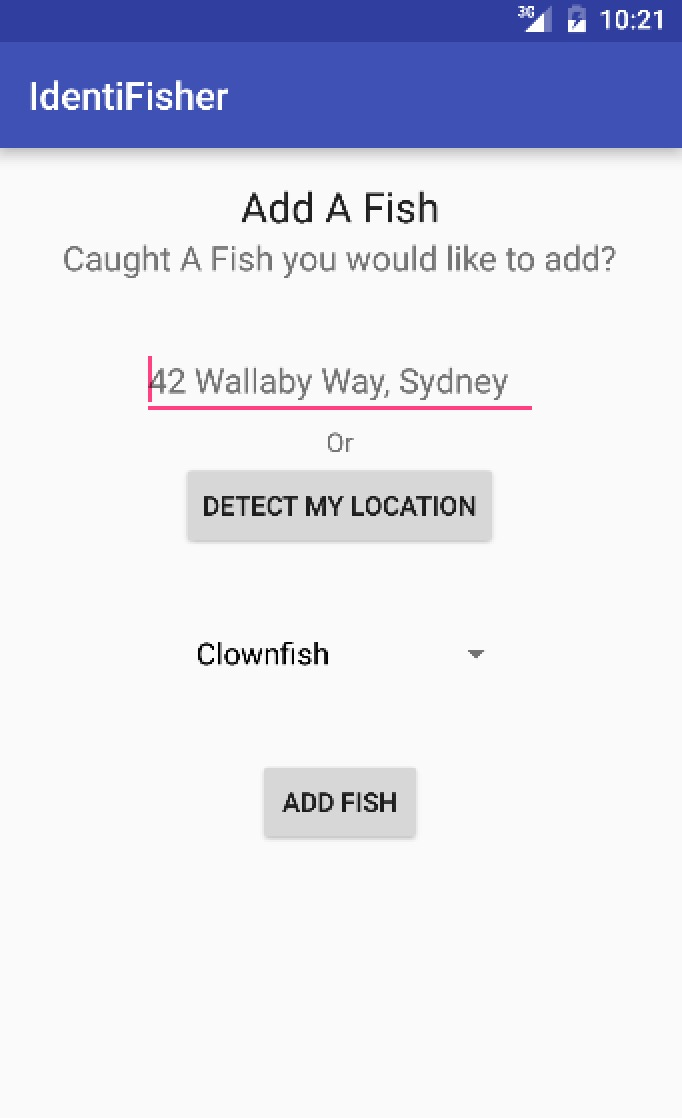
\includegraphics[scale=0.30]{AddFish.png}
	\caption{ADD A FISH page of IdentiFisher Application}
\end{figure}

\section{Examples}

\subsection{Identifying A Fish}
First, open the application and click on \textit{IDENTIFISHER}. Begin by clicking on the drop-down menus and select the most accurate attributes that describe the fish you would like to identify. After doing so, and being content with the properties, click on the Identify button. The appliation will now try to identify the fish and will list them from most likely to least likely. Congratulations! You have offically identified a fish!

\subsection{Adding an Unknown Fish to the Database}
If you haven't identified the fish, consult the previous section to learn how to do so. Once the list of possible fish is displayed, it is important to look at the most likely candidates and to choose the best one with your given knowledge. After deciding and clicking on the one you believe is correct, click Add Fish. Congratulations! You have offically identified a fish and added it to the database!

\subsection{Adding a Known Fish to the Database}
If you already know which type of fish you have caught, you may simply add it to the database without going through the identification process. In this case, navigate to the ADD A FISH page of the application, input your location textually or by selecting the DETECT MY LOCATION button. Next, you select your type of fish from the drop-down menu and click ADD FISH. Congratulations! Once screening has been performed by the database administrator, you will have successfully added a known fish to the database! 

\subsection{Looking Up Lake Statistics}
If you would like catch rate statistics about a specific lake, navigate to the LOOK UP LAKE page. Next, enter a location into the text field and click the button FIND MY LAKE. A list of fish that may be found in a lake near this location will be provided. Congratulations! You have successfully searched for lake statistics!

\section{Server Administrator Instructions}

\subsection{Swapping Experts}
In order to add an expert, follow these instructions:
\begin{itemize} 
	\item Be Sure that the Expert being added is a child class to the Expert Class in the Application
	\item Increase the size of the Expert array by 1, as seen in the ExpertManager constructor
	\item Then fill new place in array with the new Expert child object, passing on any necessary information such as the encryption key
\end{itemize}
In order to delete an expert, follow these instructions:
\begin{itemize} 
	\item Decrease the size of the Expert array by 1, as seen in the ExpertManager constructor
	\item Then delete the line where the array is filled with the Expert being deleted and shift any current Experts if necessary 
\end{itemize}

\section{Functional Requirements}
The functional requirements that were identified at the early development stages are satisfied. The following list describes the manner in which the requirements have been satisfied:

\begin{itemize} 
	\item F1.1: The application accepts the physical specifications of a fish by allowing the user to pick appropriate traits from
	drop-down menus which are then used by experts to query the database.
	\item F1.2: The application will sort all fish possible given by experts from most to least frequently with more frequently named fish having higher
	accuracy. The result will be displayed to the user in that order with no overlaps.
	\item F1.3: The user may submit the fish using the ADD FISH button or page.
	\item F2.2: The application can show the user catch rate statistics of a lake near a location using the LOOK UP LAKE page.
	\item F3.3: The application allows the user to submit their catch results using the ADD FISH page.
	\item Expert add/removal/modify: The addition, deletion, and update of experts can be done by modifying the Java code as
	described in the aforementioned section.
\end{itemize}

\newpage
\listoffigures

\end{document}
